\chapter[Metodologia]{Metodologia}

\section{Desenvolvimento do Firmware}
\subsection{Ambiente de Desenvolvimento}
O firmware foi desenvolvido para a placa WeAct ESP32-C3FH4, baseada no microcontrolador ESP32-C3 da Espressif (China), que opera com arquitetura RISC-V de 32 bits, frequência de até 160 MHz, 400 kB de RAM, 384 kB de ROM, 4 MB de FLASH e até 22 pinos GPIO programáveis \cite{weact_esp32c3}. Foi utilizada a linguagem MicroPython na versão 1.24.1, compatível com a arquitetura da placa, cuja imagem de firmware foi obtida no site oficial do projeto \cite{micropython_esp32c3_download}. A gravação do firmware e a transferência dos scripts foram realizadas por meio da Thonny IDE, comumente adotado para aplicações com MicroPython \cite{thonny_ide}.

\subsection{Estruturação do Projeto e Modularização}
A arquitetura do firmware foi organizada em três diretórios principais (\texttt{lib}, \texttt{data}, \texttt{tasks}) complementados pelo arquivo \texttt{main.py}, responsável por coordenar a inicialização do sistema. No diretório \texttt{lib}, foram alocadas bibliotecas específicas, incluindo a \texttt{aioble}, uma biblioteca recomendada pela própria documentação do MicroPython para a maioria das aplicações com Bluetooth Low Energy (BLE) \cite{micropython_ble_docs}. Essa biblioteca abstrai a complexidade das operações de conexão, emparelhamento e troca de dados via GATT, facilitando a implementação de servidores BLE no ESP32-C3 \cite{aioble_repo}. O subdiretório \texttt{utils} concentrou módulos auxiliares, como \texttt{bluetooth\_config.py}, para definição de parâmetros de conexão, e \texttt{data\_converter.py}, para serialização dos dados trocados com o aplicativo Android.

A persistência de configurações operacionais foi implementada no diretório \texttt{data} através do arquivo \texttt{config.json}, complementado por um conjunto de valores padrão em \texttt{default\_data.py} como mecanismo de segurança para cenários de corrupção de dados salvos.

\subsection{Gestão de Tarefas Assíncronas}
A lógica central do firmware foi desenvolvida no arquivo \texttt{main.py}, onde foram instanciadas cinco corrotinas principais utilizando o módulo \texttt{asyncio} do MicroPython. A função \texttt{main()} coordena:

\begin{itemize}

    \item \texttt{peripheral\_task()}, responsável pelo ciclo de vida das conexões BLE;
    \item \texttt{send\_heartbeat\_task()}, que emite pacotes de sincronização a cada 2 segundos contendo métricas de integridade do sistema utilizando o módulo utilitário \texttt{memory\_usage.py};
    \item \texttt{read\_task()}, dedicada ao processamento de dados recebidos via Bluetooth com despacho para handlers especializados;
    \item \texttt{malting\_task()}, núcleo do controle do processo de malteação.
    \item \texttt{sensors\_task()}, que gerencia a leitura periódica dos sensores instalados.


\end{itemize}

\begin{figure}[ht]
    \centering
    \caption{Esquema geral do projeto com as tarefas assíncronas em evidência}
    \label{fig:TarefasAssincronasFluxograma}
    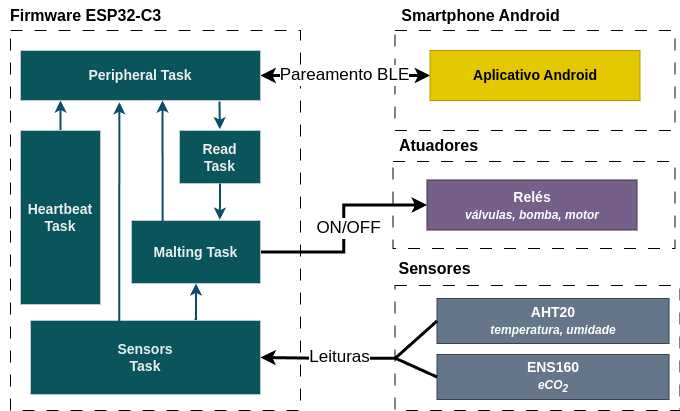
\includegraphics[width=1.0\textwidth]{TarefasAssincronas.drawio.png}

    {\centering\footnotesize Fonte: Autoria própria.\par}
\end{figure}

A tarefa \texttt{read\_task} fica aguardando o recebimento de \textit{bytes}. Quando um pacote é recebido, essa tarefa delega o tratamento dos dados para \texttt{task\_handler}, que, por sua vez, direciona os dados para outros módulos de acordo com o primeiro \textit{byte} do \textit{array} (lista). Por exemplo, ilustrado pela \autoref{fig:ReadTaskDrawio}, se o primeiro \textit{byte} for igual a 1, vai acionar o módulo de alteração dos parâmetros, que são utilizados para a realização da malteação — que é iniciada quando o \textit{array} inicia com 255.

\begin{figure}[ht]
    \centering
    \caption{Lógica do recebimento de comandos do dispositivo}
    \label{fig:ReadTaskDrawio}
    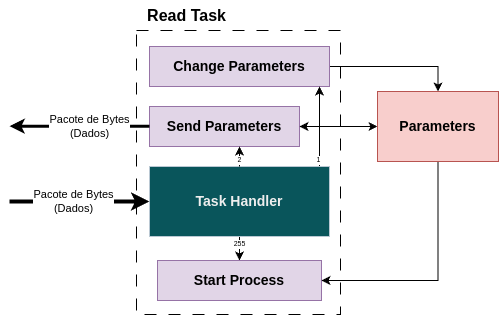
\includegraphics[width=0.7\textwidth]{ReadTask.drawio.png}

    {\centering\footnotesize Fonte: Autoria própria.\par}
\end{figure}

\subsection{Algoritmos de Controle do Processo de Malteação}
A sequência de maceração, germinação e secagem foi modelada no subdiretório \texttt{malting\_stages} em módulos especializados (\texttt{steeping.py}, \texttt{germination.py}, \texttt{kilning.py}). Cada etapa opera como uma corrotina independente, monitorando variáveis críticas com base nas condicionais dos parâmetros recebidos via Bluetooth. A estrutura assíncrona permitiu a execução não bloqueante desses processos, essencial para a continuidade da comunicação Bluetooth mesmo durante o processo. As lógicas de marcação de tempo foram desenvolvidas com o uso do módulo utilitário \texttt{uptime.py}, que se baseia no tempo total de execução do dispositivo.

\begin{figure}[ht]
    \centering
    \caption{Fluxograma do controle planejado para o algoritmo de malteação}
    \label{fig:logicamalteacao}
    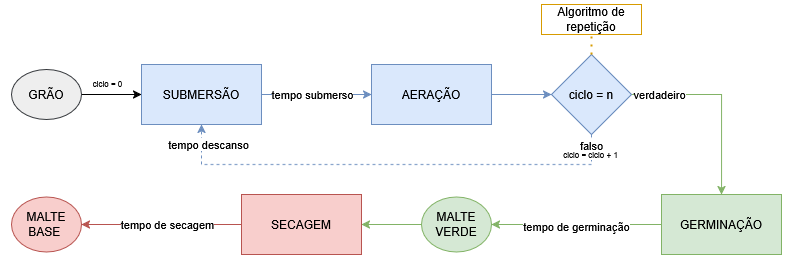
\includegraphics[width=1.0\textwidth]{logicamalteacao.png}

    {\centering\footnotesize Fonte: Autoria própria.\par}
\end{figure}

  
\section{Desenvolvimento do Aplicativo}
\subsection{Ambiente e Ferramentas de Desenvolvimento}

O ambiente de desenvolvimento foi estabelecido utilizando a IDE Android Studio (Koala Feature Drop - 2024.1.2) com linguagem Kotlin na versão 1.9.10. Os testes foram conduzidos em um dispositivo físico com Android 14, garantindo compatibilidade com as APIs mais recentes do sistema operacional. Escolheu-se o ecossistema Android Jetpack como base tecnológica devido a sua estabilidade e suporte oficial da plataforma Google para desenvolvimento de aplicativos.

\subsection{Arquitetura e Padrões de Projeto}

Adotou-se uma arquitetura em camadas conforme as diretrizes de boas práticas do Android Moderno, estruturada em três módulos principais: \textit{data}, \textit{domain} e \textit{presentation}. O módulo \textit{data} concentra a gestão de fluxos de informação, incluindo a comunicação \textit{Bluetooth} e o armazenamento local de dados, implementado com o uso das bibliotecas \textit{Room} e \textit{DataStore}. A \textit{Room} é uma biblioteca de que facilita o acesso a bancos SQLite no sistema Android \cite{android_room}. Já a \textit{DataStore} é projetada para armazenar preferências e pequenas quantidades de dados de forma mais eficiente \cite{android_datastore}.

Na camada \textit{domain}, implementou-se a lógica de negócios e o tratamento de dados. Por fim, a camada de \textit{presentation} foi construída com \textit{Jetpack Compose}, utilizando os princípios do \textit{Design Material 3} que define diretrizes de usabilidade, hierarquia visual e acessibilidade para o desenvolvimento de interfaces \cite{material3}.

\begin{figure}[ht]
    \centering
    \caption{Diagrama da arquitetura em camadas}
    \label{fig:layerarch}
    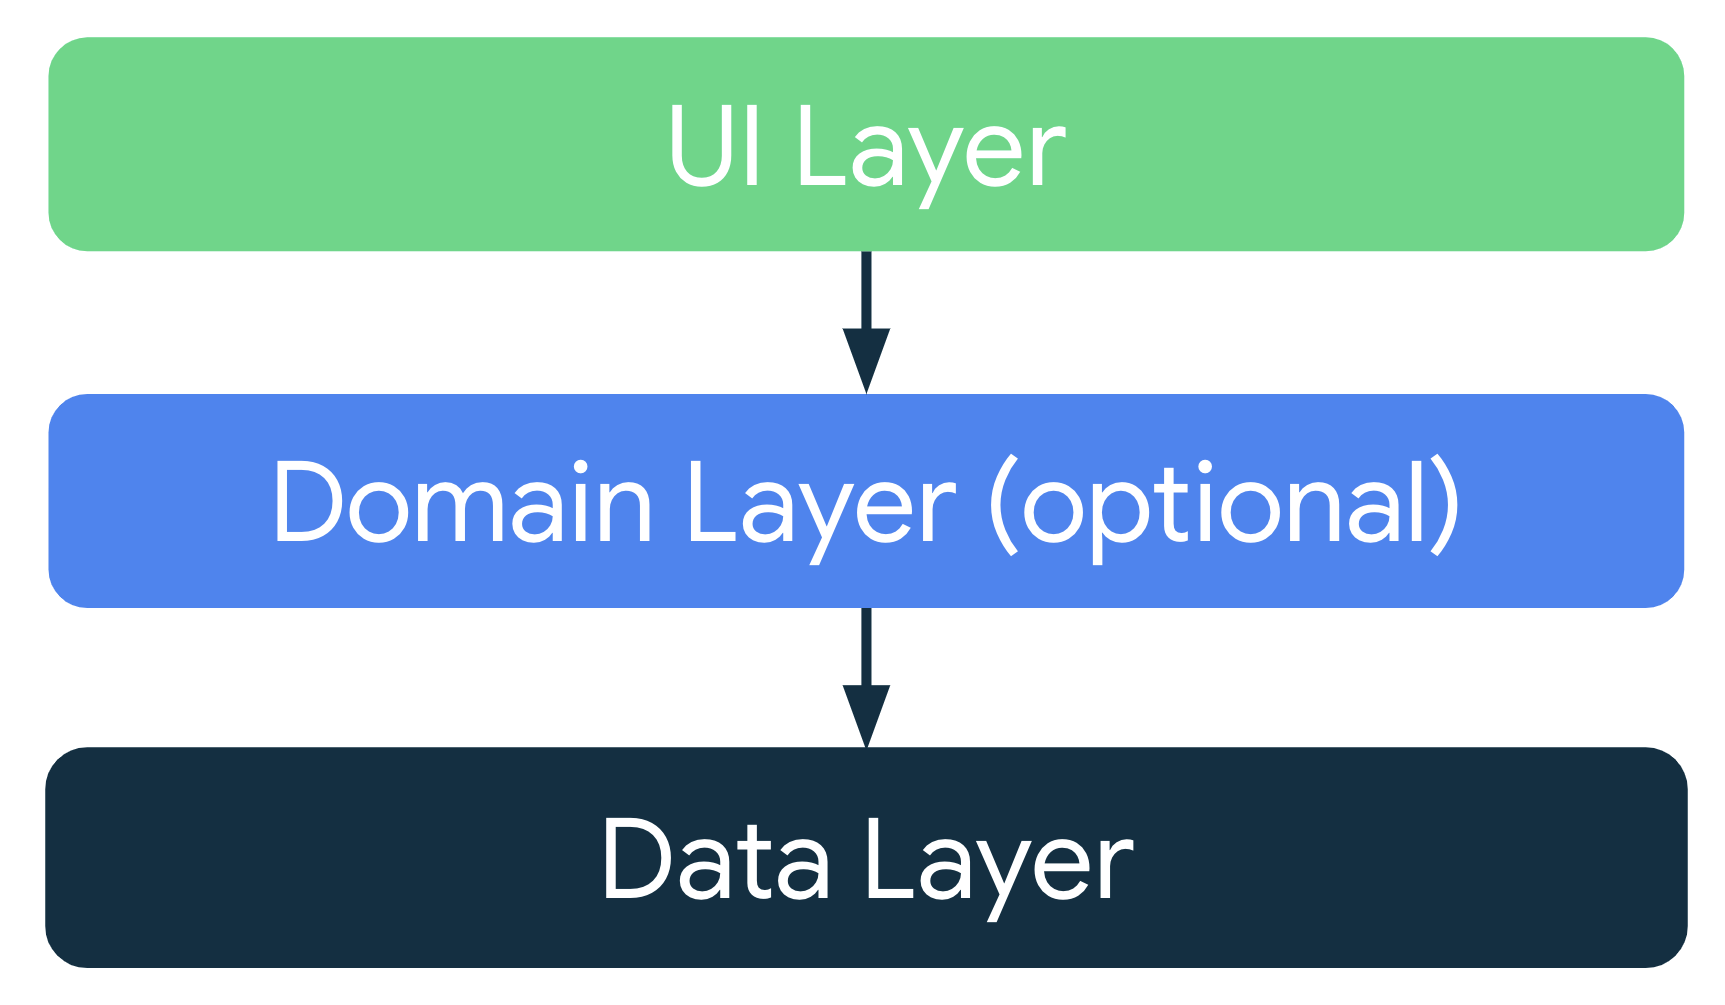
\includegraphics[width=0.6\textwidth]{layerarch.png}

    {\centering\footnotesize Fonte: Developers Android.\par}
\end{figure}

\section{Documentação}
A gestão do código foi implementada mediante a utilização do sistema de controle de versão Git, com hospedagem pública em dois repositórios GitHub dedicados: um para o firmware \url{https://github.com/NicolasDezan/ESP32C3-MaltingControl.git} e outro para o aplicativo Android \url{https://github.com/NicolasDezan/MALT-ESP.git}. A separação em repositórios distintos buscou garantir a modularidade entre os componentes de software, além de facilitar a manutenção independente de cada projeto.

% \subsection{Tutoriais}
% Talvez eu grave tutoriais mostrando os códigos e o sistema funcionando etc etc etc
% Se sobrar tempo e se os videos ficarem legais eu vou incluir uma fala do tipo:
% A documentação técnica incluiu tutoriais em vídeo externos (links no arquivo \texttt{README.md}) detalhando processos críticos como configuração inicial do ESP32-C3 e emparelhamento Bluetooth.